\chapter{Results and Discussion}
\label{chap:05}
\paragraph{}

The Runge-Kutta fourth-order method  and Euler's method can be used to optimize and improve the performance of the intracellular signalling network for the STAT1, STAT3, BCL-2 and BAX proteins. This method can be used to determine the relationship between the initial conditions and other parameters of the proteins, such as anti-tumour drugs in the presence of IFN-$\beta$ and JAK stimuli. By doing so, the dynamic characteristics of the proteins can be predicted under different conditions and calculated using the numerical method of Runge-Kutta fourth order and Euler's method. This allows for precise \cite{lee2021mathematical}imation of the proteins' dynamic characteristics during their movement processes and adequate description of the different processes under various given conditions. The results obtained using this method, such as  the presence of IFN-$\beta$ and JAK and other effective parameters, provide valuable insights into the behaviour of the STAT1, STAT3, BCL-2 and BAX proteins.


\begin{table}[hbt!]
\begin{center}
    \begin{tabular}{p{2cm}|p{6cm}|p{3cm}}
    \hline
    \textbf{Constant} & \textbf{Description of constant} & \textbf{Values}
    \\
    \hline \hline
 ${S_1}^*$&STAT1 concentration&2.42 $\mu g ml^{-1}$\\
${S_3}^*$&STAT3 concentration&1.38 $\mu g ml^{-1}$\\
$B^*$&Bcl-2 concentration&10 nM \\
$X^*$&BAX concentration&351  $\mu$M\\
$S^*$&IFN-$\beta$ concentration&10 $ng ml^{-1}$\\
$J^*$&JAK2 concentration&10 nM\\
$D^*$&DDP concentration&10 $\mu g ml^{-1}$\\
$T^*$&tumour volume&$100mm^3$\\
     \hline
    \end{tabular}
    \caption{Initial values corresponding to the STAT1, STAT3, Bcl-2, BAX and other parameters.  }
    \label{tab1}
    \end{center}
\end{table}

% For future illustration, above Table\ref{tab1} values will be used. Each iteration calculated will be calculated using step size and time. 

 \begin{table}[hbt!]
\begin{center}
    \begin{tabular}{p{2.5cm}|p{9cm}|p{1.2cm}|p{2cm}}
    \hline
  \textbf{Constant} &  \textbf{Description of constant} &\textbf{Values} &\textbf{Reference}
    \\
    \hline \hline
    S & IFN-$\beta$ signalling  & 0-1.0& \cite{lee2021mathematical,deng2014sting}\\
$k_1$ & autocatalytic production rate(STAT1 module) & 4.0 & \cite{lee2021mathematical}\\
$ k_2$ & Hill-type coefficient (STAT1 module) & 1.0  & \cite{lee2021mathematical}\\
   $\alpha$ & inhibition strength of STAT1 by STAT3 & 1.5 & \cite{lee2021mathematical}\\
   $\lambda_k $& signalling source of STAT3 & 1.0 & \cite{lee2021mathematical}\\
   $ \lambda_J$ & induction rate of STAT3 by JAK2 & 4.0 & \cite{lee2021mathematical}\\
      J & JAK2 signalling level & 0-1.0 & \cite{lee2021mathematical}\\
K & inhibition parameter & 5.0 & \cite{lee2021mathematical}\\
$k_3$ & autocatalytic production rate (STAT3 module) & 4.0 & \cite{lee2021mathematical}\\
$k_4$ & Hill-type coefficient (STAT3 module) & 1.0 & \cite{lee2021mathematical}\\
$\beta$ & inhibition strength of STAT3 by STAT1& 1.0 & \cite{lee2021mathematical}\\
$\mu_3$ & relative decay rate of STAT3 & 1.0 & \cite{andrejeva2002degradation, yang2017porcine}\\
$\lambda_1$ & signalling source of Bcl-2 & 0.2 & \cite{lee2021mathematical}\\
$k_5$ & autocatalytic production rate (Bcl-2 module) & 1.0 & \cite{lee2021mathematical}\\
$k_6$ & Hill-type coefficient (Bcl-2 module) & 1.0 & \cite{lee2021mathematical}\\
$\gamma $ & inhibition strength of Bcl-2 by STAT$1_1$ & 1.0 & \cite{lee2021mathematical}\\
$\lambda_3$ & signalling from STAT3 & 1.2 & \cite{lee2021mathematical}\\
$\mu_B$ & relative decay rate of Bcl-2 & 1.2 &  \cite{andrejeva2002degradation, yang2017porcine}\\
$\lambda_2$ & signalling source of BAX& 0.2 & \cite{lee2021mathematical}\\
$k_7$ & autocatalytic production rate (BAX module) & 4.0 & \cite{lee2021mathematical}\\
$k_8$ & Hill-type coefficient (BAX module) & 1.0 & \cite{lee2021mathematical}\\
$\Lambda$ & inhibition strength of BAX by Bcl-2& 1.0 & \cite{lee2021mathematical}\\
$\mu_X$ & relative decay rate of BAX & 5.0& \cite{magal2005downregulation, xin2005nicotine}\\
\textbf{Threshold} & & & \\ 
\hline
 ${S_1}^{th}$ & threshold of STAT1  & 1.8& \cite{lee2021mathematical}\\
 ${S_3}^{th}$ & threshold of STAT3  & 1.3& \cite{lee2021mathematical}\\
 $B^{th}$ & threshold of Bcl-2  & 1.44& \cite{lee2021mathematical}\\
 $X^{th}$ & threshold of BAX  & 0.3& \cite{lee2021mathematical}\\
\textbf{Tumour module} & & &\\
     \hline
 r& growth rate of tumour cells& 0.12&\cite{catani2016intratumoral}\\
 ${k_9}$& inhibition parameter of STAT1 growth& 1.0&\cite{catani2016intratumoral}\\
 ${k_{10}}$& inhibition parameter of STAT1 growth& 10&\cite{catani2016intratumoral}\\
 ${T_0}$& carrying capacity of a tumour&100&\cite{catani2016intratumoral}\\
${\mu_T}$& killing rate of tumour cells by apoptosis&0.1&\cite{catani2016intratumoral}\\
 \hline
    \end{tabular}
    \caption{Values of the constant corresponding to the mathematical model. }
    \label{tabR1}
    \end{center}
\end{table}

Dynamic behaviour of STAT1, STAT3, BCL-2, and BAX systems optimized and analyzed using Runge-Kutta and Euler's method using Table \ref{tabR1} and Table \ref{tabR2}.

\newpage


 \begin{table}[hbt!]
\begin{center}
    \begin{tabular}{p{2.5cm}|p{6cm}|p{2cm}|p{2cm}}
    \hline
  \textbf{Constant} &  \textbf{Description of constant} &\textbf{Values} &\textbf{Reference}
    \\
    \hline \hline
\textbf{Therapeutics}& & &\\
 ${\mu_S}$& decay rate of IFN-$\beta$ &4.8& \cite{salmon1996pharmacokinetics}\\
 ${J_s}$& source of JAK2&1.3& \cite{lin2008fc}\\
 ${\mu_J}$& decay rate of JAK2 &1.3& \cite{lin2008fc}\\
 ${\gamma_D}$& degradation rate of JAK2 by DDP &1.0& \cite{lee2021mathematical}\\
     ${\mu_D}$&decay rate of DDP &10& \cite{crom1981cisplatin}\\
\textbf{Reference value}& & &\\
${S_1}^*$&STAT1 concentration&2.42 $\mu g ml^{-1}$& \cite{liu2014active}\\
${S_3}^*$&STAT3 concentration&1.38 $\mu g ml^{-1}$&\cite{liu2014active}\\
$B^*$&Bcl-2 concentration&10 nM & \cite{vickers2017animal}\\
$X^*$&BAX concentration&351  $\mu$M &\cite{vickers2017animal}\\
$S^*$&IFN-$\beta$ concentration&10 $ng ml^{-1}$& \cite{yu2009transcriptional}\\
$J^*$&JAK2 concentration&10 nM& \cite{lee2021mathematical,yu2009transcriptional}\\
$D^*$&DDP concentration&10 $\mu g ml^{-1}$&\cite{lee2021mathematical}\\
$T^*$&tumour volume&$100mm^3$&\cite{lee2021mathematical}\\
 \hline
    \end{tabular}
    \caption{Values of the constant corresponding to the mathematical model.}
    \label{tabR2}
    \end{center}
\end{table}


\section{Numerical results for $S =0$ and $J=0$}
\paragraph{}

This section discusses the behaviour of intracellular modules (STAT1, STAT3, Bcl-2, and BAX) using Euler's method and Runge Kutta fourth-order method. The behaviour of each module is depicted in figures, with solid, dashed, dotted, and dot-dashed lines representing STAT1, STAT3, Bcl-2, and BAX, respectively. Comparison results for each module are also shown in separate figures for clarity. The dynamics of STAT1, STAT3, and Bcl-2 are consistent with the numerical results of both Euler's and the Runge Kutta methods.

In Figure \ref{r2} the behaviour of intracellular module (STAT1, STAT3, Bcl-2, and BAX) using Runge kutta fourth order method. Using Figues \ref{r1} and Figure \ref{r2} it is challenging to refer to changes in their behaviours. Therefore, comparison result of each module (STAT1, STAT3, Bcl-2, and BAX) can be shown in Figures \ref{r3}, \ref{r4}, \ref{r5} and \ref{r6}. The dynamics of STAT1  (Figure \ref{r3}) STAT3  (Figure \ref{r4}) and Bcl-2 (Figure \ref{r5}) have coincided of their results corresponding to the numerical result of Runge Kutta method and Euler's method.  

\begin{figure}[hbt!]
	\centering
	\begin{framed}
	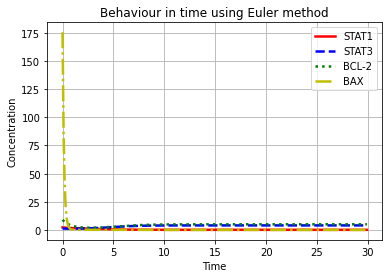
\includegraphics[width=0.68\textwidth]{Figures/A/N1.png}
		\end{framed}
	\caption{Numerical results by Euler's method when $S =0$ and $J=0$.}
	\label{r1}
\end{figure}


\begin{figure}[hbt!]
	\centering
	\begin{framed}
	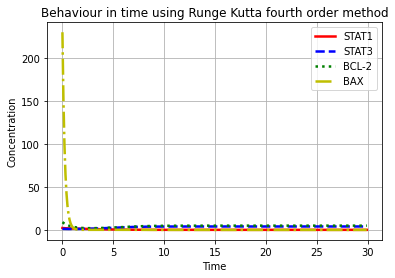
\includegraphics[width=0.68\textwidth]{Figures/A/N2.png}
		\end{framed}
	\caption{Numerical results by Runge kutta fourth order method  when $S =0$ and $J=0$. }
	\label{r2}
\end{figure}

\begin{figure}[hbt!]
	\centering
	\begin{framed}
	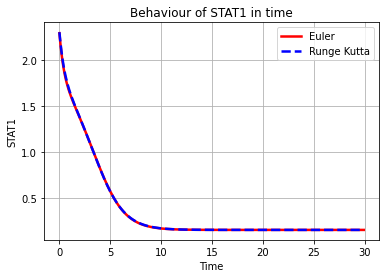
\includegraphics[width=0.68\textwidth]{Figures/A/N3.png}
		\end{framed}
	\caption{STAT1 behavior corresponding to the RK4 method and Euler's method  when $S =0$ and $J=0$.}
	\label{r3}
\end{figure}
 
\begin{figure}[hbt!]
	\centering
	\begin{framed}
	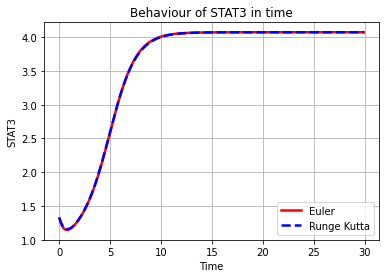
\includegraphics[width=0.67\textwidth]{Figures/A/N4.png}
		\end{framed}
	\caption{STAT3 behavior corresponding to the RK4 method and Euler's method  when $S =0$ and $J=0$.}
	\label{r4}
\end{figure}

\begin{figure}[hbt!]
	\centering
	\begin{framed}
	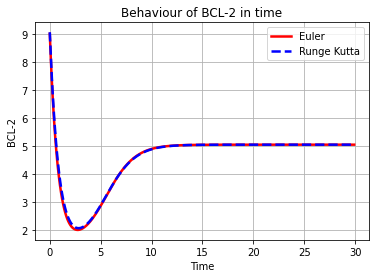
\includegraphics[width=0.67\textwidth]{Figures/A/N5.png}
		\end{framed}
	\caption{Bcl-2 behavior corresponding to the RK4 method and Euler's method  when $S =0$ and $J=0$.}
	\label{r5}
\end{figure}

\begin{figure}[hbt!]
	\centering
	\begin{framed}
	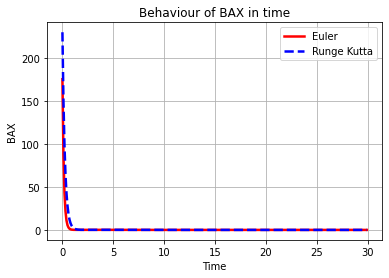
\includegraphics[width=0.67\textwidth]{Figures/A/N6.png}
		\end{framed}
	\caption{BAX behavior corresponding to the RK4 method and Euler's method  when $S =0$ and $J=0$.}
	\label{r6}
\end{figure}





\section{Numerical results for $S =0.4$ and $J=0$}
\paragraph{}
 
In this section, there are several scenarios will be discussed with analysis results. Results will be interpreted corresponding to the $S =0.4$ and $J=0$  values and initial values as given in Table \ref{tab1}. Figure \ref{r13} depicts the behaviour of the intracellular module (STAT1, STAT3, Bcl-2, and BAX) using Euler's method and Runge kutta fourth order method. Each and every intracellular module (STAT1, STAT3, Bcl-2, and BAX) starts in different initial conditions and then they are decremented into several values. The solid, dashed, dotted, and dot-dashed lines represent the STAT1, STAT3, Bcl-2, and BAX, respectively. 

In Figure \ref{r14} the behaviour of intracellular module (STAT1, STAT3, Bcl-2, and BAX) using Runge kutta fourth order method. Using Figues \ref{r13} and Figure \ref{r14}, it is challenging to refer to changes in their behaviours. Therefore, comparison result of each module (STAT1, STAT3, Bcl-2, and BAX) can be shown in Figures \ref{r15}, \ref{r16}, \ref{r17} and \ref{r18}. The dynamics of STAT1  (Figure \ref{r15}) STAT3  (Figure \ref{r16}) and Bcl-2 (Figure \ref{r17}) have coincided with their results corresponding to the numerical result of Runge Kutta method and Euler's method.

 \begin{figure}[hbt!]
	\centering
	\begin{framed}
	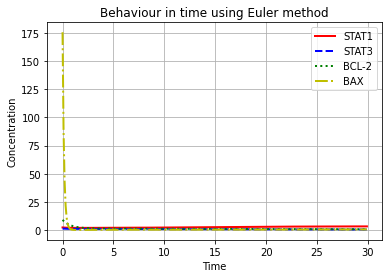
\includegraphics[width=0.68\textwidth]{Figures/C/N1.png}
		\end{framed}
	\caption{Numerical results  by Euler's method when $S =0.4$ and $J=0$.}
	\label{r13}
\end{figure}

\begin{figure}[hbt!]
	\centering
	\begin{framed}
	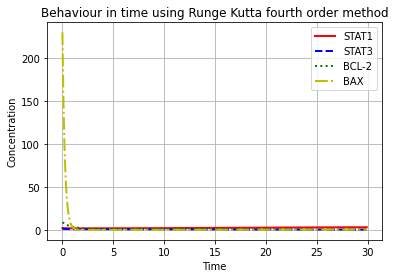
\includegraphics[width=0.68\textwidth]{Figures/C/N2.png}
		\end{framed}
	\caption{Numerical results  by Runge kutta fouth order method when $S =0.4$ and $J=0$. }
	\label{r14}
\end{figure}

\begin{figure}[hbt!]
	\centering
	\begin{framed}
	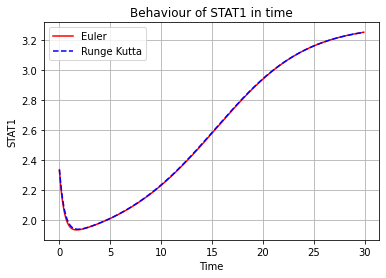
\includegraphics[width=0.68\textwidth]{Figures/C/N3.png}
		\end{framed}
	\caption{STAT1 behavior corresponding to the RK4 method and Euler's method when $S =0.4$ and $J=0$.}
	\label{r15}
\end{figure}

\begin{figure}[hbt!]
	\centering
	\begin{framed}
	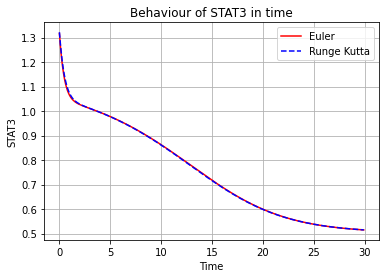
\includegraphics[width=0.68\textwidth]{Figures/C/N4.png}
		\end{framed}
	\caption{STAT3 behavior corresponding to the RK4 method and Euler's method when $S =0.4$ and $J=0$.}
	\label{r16}
\end{figure}

\begin{figure}[hbt!]
	\centering
	\begin{framed}
	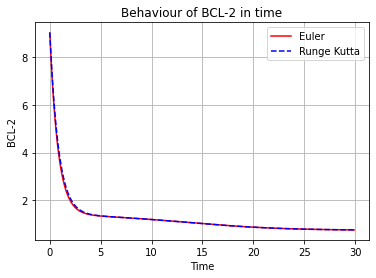
\includegraphics[width=0.68\textwidth]{Figures/C/N5.png}
		\end{framed}
	\caption{Bcl-2 behavior corresponding to the RK4 method and Euler's method when $S =0.4$ and $J=0$.}
	\label{r17}
\end{figure}

\begin{figure}[hbt!]
	\centering
	\begin{framed}
	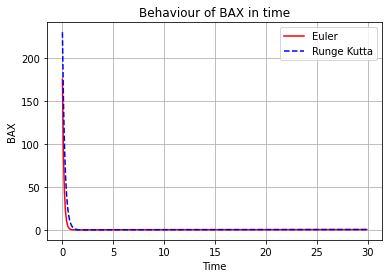
\includegraphics[width=0.68\textwidth]{Figures/C/N6.png}
		\end{framed}
	\caption{BAX behavior corresponding to the RK4 method and Euler's method when $S =0.4$ and $J=0$.}
	\label{r18}
\end{figure}

\section{Numerical results for $S =1$ and $J=1$}
\paragraph{}


In this section, the presence of both IFN-$\beta$ signalling and JAK2 signalling levels will be examined through analysis of results. The interpretation of the results will be based on the values of $S=1$ and $J=1$ as listed in Table 1. Figures \ref{r19}  and \ref{r20}  show the behaviour of the intracellular modules (STAT1, STAT3, Bcl-2, and BAX) using both Euler's method and the Runge-Kutta fourth-order method, respectively. The initial conditions for each of the modules were set as given in Table \ref{tab1}. The figures' solid line, dashed line, dotted line, and dot-dashed line represent the behaviour of STAT1, STAT3, Bcl-2, and BAX, respectively. To better understand the changes in their behaviour, comparison results for each module can be found in Figures \ref{r21}, \ref{r22}, \ref{r23} and \ref{r24}. The dynamics of STAT1  (Figure \ref{r21}) STAT3  (Figure \ref{r22}) and Bcl-2 (Figure \ref{r23}) have coincided of their results corresponding to the numerical result of Runge-Kutta method and Euler's method. The dynamics of STAT1, STAT3, and Bcl-2 are consistent with the numerical results obtained from both Runge-Kutta and Euler's method.  

\newpage

 \begin{figure}[hbt!]
	\centering
	\begin{framed}
	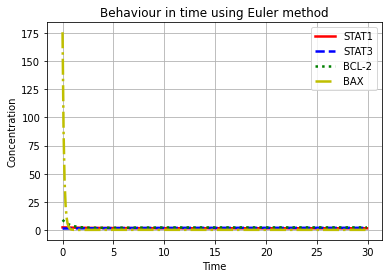
\includegraphics[width=0.68\textwidth]{Figures/D/N1.png}
		\end{framed}
	\caption{Numerical results  by Euler's method when $S =1$ and $J=1$.}
	\label{r19}
\end{figure}

\begin{figure}[hbt!]
	\centering
	\begin{framed}
	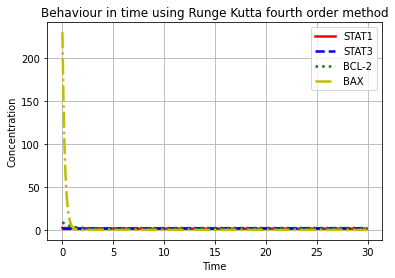
\includegraphics[width=0.68\textwidth]{Figures/D/N2.png}
		\end{framed}
	\caption{Numerical results  by Runge kutta fouth order method when $S =1$ and $J=1$. }
	\label{r20}
\end{figure}

\begin{figure}[hbt!]
	\centering
	\begin{framed}
	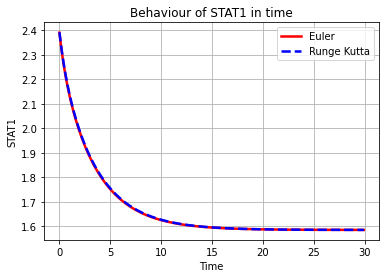
\includegraphics[width=0.68\textwidth]{Figures/D/N3.png}
		\end{framed}
	\caption{STAT1 behavior corresponding to the RK4 method and Euler's method when $S =1$ and $J=1$.}
	\label{r21}
\end{figure}

\begin{figure}[hbt!]
	\centering
	\begin{framed}
	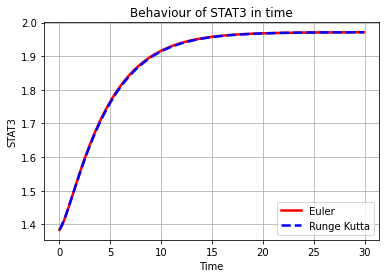
\includegraphics[width=0.68\textwidth]{Figures/D/N4.png}
		\end{framed}
	\caption{STAT3 behavior corresponding to the RK4 method and Euler's method when $S =1$ and $J=1$.}
	\label{r22}
\end{figure}

\begin{figure}[hbt!]
	\centering
	\begin{framed}
	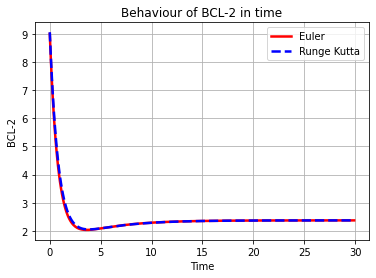
\includegraphics[width=0.68\textwidth]{Figures/D/N5.png}
		\end{framed}
	\caption{Bcl-2 behavior corresponding to the RK4 method and Euler's method when $S =1$ and $J=1$.}
	\label{r23}
\end{figure}

\begin{figure}[hbt!]
	\centering
	\begin{framed}
	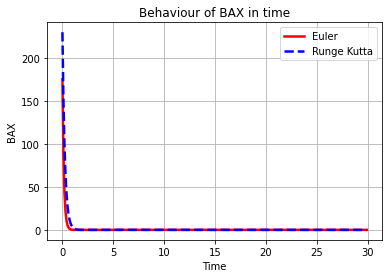
\includegraphics[width=0.68\textwidth]{Figures/D/N6.png}
		\end{framed}
	\caption{BAX behavior corresponding to the RK4 method and Euler's method when $S =1$ and $J=1$.}
	\label{r24}
\end{figure}

\section{Equilibrium and stability analysis}
\paragraph{}

This section will be described the equilibrium and stability analysis
corresponding to the mathematical model. 

considering the Jacobean matrix for the equations, 

\begin{equation}
\label{s1}
    J = \begin{bmatrix}
\frac{\partial H1}{\partial S1} & \frac{\partial H1}{\partial S3} & \frac{\partial H1}{\partial B} & \frac{\partial H1}{\partial X} \\
\frac{\partial H2}{\partial S1} & \frac{\partial H2}{\partial S3} & \frac{\partial H2}{\partial B} & \frac{\partial H2}{\partial X} \\
\frac{\partial H3}{\partial S1} & \frac{\partial H3}{\partial S3} & \frac{\partial H3}{\partial B} & \frac{\partial H3}{\partial X} \\
\frac{\partial H4}{\partial S1} & \frac{\partial H4}{\partial S3} & \frac{\partial H4}{\partial B} & \frac{\partial H4}{\partial X}
\end{bmatrix}
\end{equation}

\begin{equation}
\label{se2}
    J = \begin{bmatrix}
-1 & -\frac{2k_1k_2^2\alpha SE_3^2}{(k_2^2 + \alpha(S_3^E)^2)^2} & 0 & 0 \\
-\frac{2k_3k_4^2\beta S_1^E}{(k_4^2+\beta(S_1^E)^2)^2} & -1 & 0 & 0 \\
-\frac{2k_5k_6^2\gamma(S_1^E)}{(k_6^2+\gamma (S_1^E)^2)} & -\lambda_3 & -\mu_B & 0 \\
0 & 0 & -\frac{2k_7k_8^2\Lambda B^E}{(k_8^2+\Lambda(B^E)^2)^2} & -\mu_X
\end{bmatrix}
\end{equation}

Then, the characteristic polynomial is given by

\begin{equation}
\label{s3}
    (J - \Lambda I) = (\Lambda + \mu_B)(\Lambda + \mu_X) (\Lambda^2 + 2\Lambda +1 - \frac{2k_1k_2^2\alpha SE_3^2}{(k_2^2 + \alpha(S_3^E)^2)^2} \times \frac{2k_3k_4^2\beta S_1^E}{(k_4^2+\beta(S_1^E)^2)^2})
\end{equation}

Where I is the identity matrix. By suing above equations \eqref{s1}. \eqref{s2} and \eqref{s3} we can determine the stability of the system. We get two real eigenvalues $(\Lambda_1 = -\mu_B < 0$ and $\Lambda_2 = - \mu_X < 0)$. And remaining two real eigenvalues are,

\begin{equation}
    \Lambda_{3,4} = -1 \pm \sqrt{\frac{2k_1k_2^2\alpha SE_3^2}{(k_2^2 + \alpha(S_3^E)^2)^2} \times \frac{2k_3k_4^2\beta S_1^E}{(k_4^2+\beta(S_1^E)^2)^2}}
\end{equation}

If $\frac{2k_1k_2^2\alpha SE_3^2}{(k_2^2 + \alpha(S_3^E)^2)^2} \times \frac{2k_3k_4^2\beta S_1^E}{(k_4^2+\beta(S_1^E)^2)^2} < 1$ the eigenvalues $\Lambda_{3,4}$ are negative and the equilibrium is stable. And also, if if $\frac{2k_1k_2^2\alpha SE_3^2}{(k_2^2 + \alpha(S_3^E)^2)^2} \times \frac{2k_3k_4^2\beta S_1^E}{(k_4^2+\beta(S_1^E)^2)^2} > 1$  then $\Lambda_{3,4} > 0$ and the equilibrium is unstable. 

By substituting parameter values in the model to \eqref{se2} , we get,

\begin{equation}
    \label{re1}
     J = \begin{bmatrix}
-1 & -\frac{12 SE_3^2}{(1 + 1.5(S_3^E)^2)^2} & 0 & 0 \\
-\frac{8 S_1^E}{(1+(S_1^E)^2)^2} & -1 & 0 & 0 \\
-\frac{2(S_1^E)}{(1+\gamma (S_1^E)^2)} & 1.2 & -1.2 & 0 \\
0 & 0 & -\frac{8 B^E}{(1+\Lambda(B^E)^2)^2} & -5
\end{bmatrix}
\end{equation}

By setting $A =  -\frac{12 SE_3^2}{(1 + 1.5(S_3^E)^2)^2}$, $B = -\frac{8 S_1^E}{(1+(S_1^E)^2)^2} $, $C = -\frac{2(S_1^E)}{(1+\gamma (S_1^E)^2)} $ and $D =  -\frac{8 B^E}{(1+\Lambda(B^E)^2)^2}$

\begin{equation}
    \label{re1}
     J = \begin{bmatrix}
-1 & A& 0 & 0 \\
B & -1 & 0 & 0 \\
C & 1.2 & -1.2 & 0 \\
0 & 0 &D & -5
\end{bmatrix}
\end{equation}

Then, the characteristic equation is

\begin{equation}
    (J - \Lambda I) = (\Lambda + \mu_B)(\Lambda + \mu_X) (\Lambda^2 + 2\Lambda +1 - AB)
\end{equation}

When $S= 0$, $(S_1^E, S_3^E.B^E, X^E) \approx (0.1519, 4.1098, 5.0910, 0.0698)$. Thus, $A \approx 1.1610, B \approx  1.1610$ and $AB \approx  0.0825 < 1$. Therefore, when $S = 0$, the equilibrium point is stable.

When $S = 1$, $A \approx  3.0568, B \approx 0.0895$, and $AB \approx 0.2736 < 1$ . 

 There are three equilibrium points when $S = 0.4$. Two steady states $(S_1^E,S_3^E.B^E,X^E) \approx (3.1415, 0.5532, 0.7965, 0.5294)$ and $(S_1^E,S_3^E.B^E,X^E) \approx (0.6991, 2.8719, 3.5983, 0.0974)$ because both $AB \approx  0.6633 < 1$ and $AB \approx 0.4863 < 1 $ respectively. When consider the  third equilibrium point $(S_1^E,S_3^E.B^E,X^E) \approx  (1.8920, 1.0586, 1.4072, 0.2084)$  is unstable with $AB \approx  1.2755 > 1$.





